%%%%%%%%%%%%%%%%%%%%%%% file template.tex %%%%%%%%%%%%%%%%%%%%%%%%%
%
% This is a general template file for the LaTeX package SVJour3
% for Springer journals.          Springer Heidelberg 2010/09/16
%
% Copy it to a new file with a new name and use it as the basis
% for your article. Delete % signs as needed.
%
% This template includes a few options for different layouts and
% content for various journals. Please consult a previous issue of
% your journal as needed.
%
%%%%%%%%%%%%%%%%%%%%%%%%%%%%%%%%%%%%%%%%%%%%%%%%%%%%%%%%%%%%%%%%%%%
%
%
\RequirePackage{fix-cm}
%
%\documentclass{svjour3}                     % onecolumn (standard format)
\documentclass[smallcondensed]{svjour3}     % onecolumn (ditto)
%\documentclass[smallextended]{svjour3}       % onecolumn (second format)
%\documentclass[twocolumn]{svjour3}          % twocolumn
%
\smartqed  % flush right qed marks, e.g. at end of proof
%
\usepackage{graphicx}
%
%\usepackage{mathptmx}      % use Times fonts if available on your TeX system
%
% insert here the call for the packages your document requires
%\usepackage{latexsym}
% etc.
%
% please place your own definitions here and don't use \def but
% \newcommand{}{}
%
% Insert the name of "your journal" with
\journalname{Journal of Global Optimization}
%
\begin{document}

\title{Parallel global optimization on GPU 
	\thanks{The revised version of the paper was supported by the Russian Science Foundation, project No 15-11-30022 ``Global optimization, supercomputing computations, and applications''}
}
%\subtitle{Do you have a subtitle?\\ If so, write it here}
%\titlerunning{Short form of title}        % if too long for running head

\author{Konstantin Barkalov         \and
        Victor Gergel 
}

%\authorrunning{Short form of author list} % if too long for running head

\institute{K. Barkalov  \at
              Computational Mathematics and Cybernetics Faculty, Lobachevsky State University of Nizhni Novgorod, Nizhni Novgorod, Russia \\
              Tel.: +7-831-4623356\\
              Fax: +7-831-4623085\\
              \email{barkalov@vmk.unn.ru} 
           \and
           V. Gergel \at
							\email{gergel@unn.ru} 
}

\date{Received: date / Accepted: date}
% The correct dates will be entered by the editor


\maketitle

\begin{abstract}
This work considers a parallel algorithm for solving multidimensional multiextremal optimization problems. This algorithm uses Peano-type space filling curves for dimension reduction. Conditions of non-redundant parallelization of the algorithm are considered. Efficiency of the algorithm on modern computing systems with the use of graphics processing units (GPUs) is investigated. Speedup of the algorithm using GPU as compared with the same algorithm implemented on CPU only is demonstrated experimentally. Computational experiments are carried out on a series of several hundred multidimensional multiextremal problems.
\keywords{Global optimization \and Parallel computing \and Graphics processing unit \and Peano-type space filling curves \and Characteristical algorithms}
% \PACS{PACS code1 \and PACS code2 \and more}
% \subclass{MSC code1 \and MSC code2 \and more}
\end{abstract}

\section{Introduction} \label{intro}

This paper considers parallel algorithms for solving multiextremal optimization problems. The objective function in such problems has several local optima (usually their number is not known and can be large). 
%new text begin
In such problems a reliable estimation of the global optimum is possible only with an a priori information about the function, allowing to estimate lower bound of the objective function using known values at search points. 
%new text end
Very often, such information is presented as the assumption that the objective function satisfies a Lipschitz condition with an a priori unknown constant $L$. 
%new text begin
The important feature of the global optimization problems is that the objective function is commonly not given by an analytical formula. The usual way to calculate the function value is to apply a computer-aided algorithm. Thus, each such calculation may be interpreted as running some blackbox device  to produce the outcome for the preset input. These runs could require substantial computer resources and therefore should not be too numerous. 
%new text end
%new word - such
Such problems are common in applications (problems of optimal design of objects and technological processes in various fields of technology, problems of model fitting according to observed data in scientific research, optimization of control processes, etc., see the review \cite{RefPinter}).

Multiextremal optimization problems offer little in terms of analytical solution, while numerical solution is computationally challenging as computational costs often grow exponentially in dimension. Using modern parallel computational systems it is possible to broaden the area of applicability of global optimization methods. At the same time, the problem of efficient parallelization of the global search process arises. Therefore, development of efficient parallel methods for numerical solution of multiextremal optimization problems and implementation of corresponding software for modern computational systems is the obvious focus of research in this area.

One of the promising trends in the field of parallel global optimization (as in many areas connected with software implementation of complex algorithms) is the use of graphics processing units (GPUs). During the last decade, productivity of GPUs has been rapidly increasing to satisfy the continuously growing demand of graphic application developers. Furthermore, some principles of development of graphics hardware have changed over the past few years. Today a GPU is a high-performance flexibly programmable and massively parallel processor that can provide solution to many computationally intensive problems \cite{RefHwu}.

%new text begin
By now, parallel implementations have been suggested for most of the existing sequential algorithms. A review of modern methods of parallel global optimization can be found, for example, in \cite{RefApuzzo}. The methods described in \cite{RefApuzzo} can be divided into two classes: deterministic methods of global optimization, and heuristic methods, which are based one way or another on the random search concept. Algorithms, which belong to the latter class, allow the use of massive parallelism and are easily implemented on GPU (see works \cite{RefFerreiro,RefZhu,RefGarcia,RefMussi} and the review \cite{RefLangdon}). Owing to their stochastic nature, algorithms of this type can guarantee convergence to a globally optimal solution only in probabilistic sense, and that sets them apart from deterministic methods.

Some parallel variants are proposed for deterministic algorithms of Lipschitzian global optimization in \cite{RefGergel2005,RefEvtushenko,RefHe,RefPaulavicius}. However, these versions of algorithms are parallelized on a computing cluster with distributed memory using multi-core CPU; implementations of Lipschitzian global optimization algorithms on GPU have not been suggested yet. For example, parallelization of algorithms based on the ideas of the branch and bound method is carried out for a small number of nodes using OpenMP and MPI technologies \cite{RefPaulavicius}. It is noteworthy that the branch and bound method is applied in other areas of optimization; in particular, combinatorial optimization and integer programming. Using GPU shows good results in these areas \cite{RefBoukedjar,RefCarneiro}. It is explained by the following factor. Problems of this class (such as the Travelling Salesman Problem or the Knapsack Problem) are characterized by short time of objective function value calculation at one point and, at the same time, relatively long time required to process the results. Therefore, the most of labor-intensive operations here consist in branching and bound computations, which are implemented on GPU (see \cite{RefBoukedjar,RefCarneiro}).

This paper considers the problems of Lipschitzian global optimization that are frequently encountered in applications. They are characterized by a considerable time required to calculate the function value at one point (in comparison with the processing of the results of such calculation). For example, the objective function can be defined by solving SLAE, ODE, PDE, or Monte Carlo simulation. Currently, GPU can be used to solve all these types of problems. 
%rev4 text begin
Moreover, a set of problems can be solved on GPU simultaneously. For example, algorithm of solving of a large amount of independent SLAE on GPU is considered in \cite{RefKindratenko}, chapter 5. Results of simultaneously solving $2 \cdot 10^4$ systems of variable size are presented. Algorithm of parallel integration of large numbers of independent ODE systems on GPU is discussed in \cite{RefKindratenko}, chapter 8. Experimental results that show good speedup in solving a set (from $10^3$ up to $10^5$) of independent ODE systems are presented. Assuming that the objective function in global optimization problem is given as SLAE or ODE system many function values can be computed simultaneously.
%rev4 text end

Therefore, calculation of an objective function values can be done using a GPU, and the main goal of the algorithm	 (working at CPU) is to efficiently select points of parallel trials. The article contains the results of an investigation into the GPU implementation of the global search parallel algorithm developed according to the information-statistical approach presented in the monograph \cite{RefStrongin2000}. Some preliminary results of research in this area have been published in \cite{RefLebedevBarkalov}.
%new text end

The main part of the paper has the following structure. Section \ref{sec:2} contains a description of the basic algorithm of global search. Section \ref{sec:3} describes a scheme of its parallelization, and section \ref{sec:4} includes theoretical statements that characterize the speedup and non-redundancy of the parallel algorithm. In section \ref{sec:5}, ways of possible implementation of the parallel algorithm on GPU are discussed. Section \ref{sec:6} contains the results of numerical experiments; a comparison of the sequential algorithm and parallel CPU and GPU versions for solving a series of test multidimensional multiextremal problems is also made. Section \ref{sec:7} concludes the paper.

\section{Multidimensional global search algorithm} \label{sec:2}

Let us consider the problem of search for a global minimum of an $N$-dimensional function $\varphi(y)$ within a hyperinterval $D$
\begin{eqnarray}\label{eq:1}
& \varphi(y^\ast)=\min{\left\{\varphi(y):y\in D\right\}},\\
& D=\left\{y\in R^N: a_i\leq y_i \leq b_i, 1\leq i \leq N\right\}. \nonumber
\end{eqnarray}

Let us assume that the function $\varphi$ satisfies a Lipschitz condition with an a priori unknown constant $L$
\[
\left|\varphi(y_1)-\varphi(y_2)\right|\leq L\left\|y_1-y_2\right\|,\; y_1,y_2 \in D,\; 0<L<\infty.
\]

There is a number of ways to adapt effective one-dimensional algorithms for solving multidimensional problems; see, for example, the diagonal partitions method in \cite{RefSergeyev2006} or the simplicial partitions method in \cite{RefZilinskas}. In this paper, we will use the approach based on the idea of dimension reduction by means of a Peano curve $y(x)$, which continuously and unambiguously maps the unit interval [0,1] onto the $n$-dimensional cube
\[
\left\{y\in R^N: -2^{-1}\leq y_i \leq 2^{-1}, 1 \leq i \leq N\right\}=\left\{y(x):0\leq x \leq 1 \right\}.
\]
%new text begin
Problems of numerical construction of Peano-type space filling curves and the corresponding theory are considered in detail in \cite{RefStrongin2000}, \cite{RefSergeyev2013}.  
%new text begin
Here we will note that a numerically constructed curve (\textit{evolvent}) is $2^{-m}$ accurate approximation of the theoretical Peano curve in $L_\infty$ metric, where $m$ is an evolvent construction parameter. Examples of the evolvent with different $m$ in two dimensions are given in Fig.~\ref{fig:0}.

%Here we will note that a numerically constructed curve (\textit{evolvent}) is an approximation to a theoretical Peano curve with an accuracy $2^{-m}$ , where $m$ is an evolvent construction parameter. It means that using an evolvent we can distinguish points in a multidimensional space, the coordinates of which differ by not less than $2^{-m}$; closer points are considered as coincident. Thereby an evolvent constructed with a fixed $m$ allows obtaining a solution of a problem with an accuracy of not more than $2^{-m}$ by coordinate. 

\begin{figure}[ht]
\begin{minipage}{0.32\linewidth}
\center{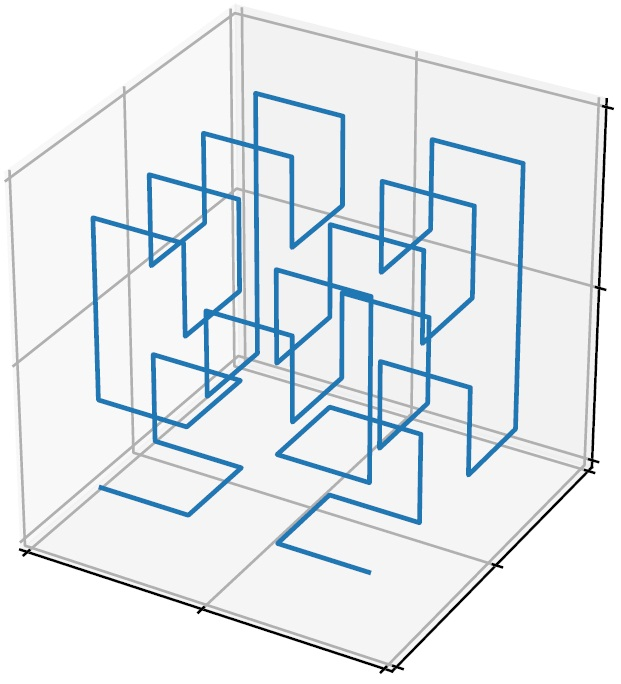
\includegraphics[width=1.0\linewidth]{fig1a.JPG} \\ (a)}
\end{minipage}
\begin{minipage}{0.32\linewidth}
\center{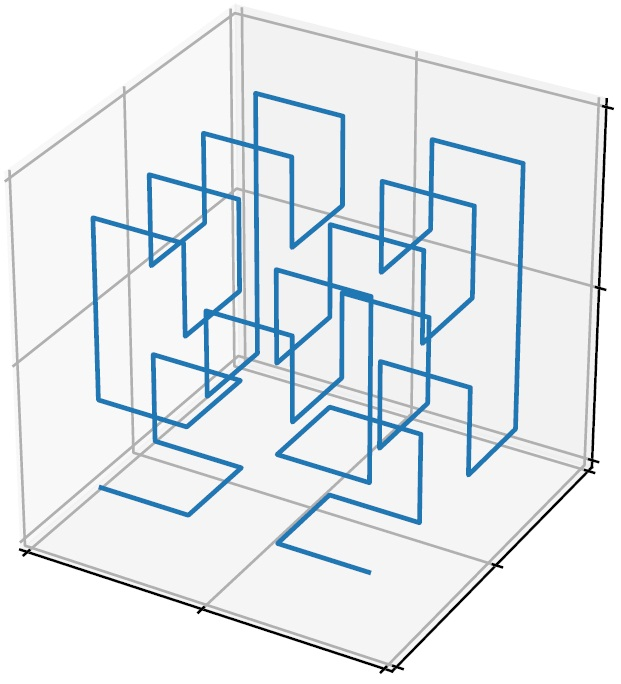
\includegraphics[width=1.0\linewidth]{fig1b.JPG} \\ (b)}
\end{minipage}
\begin{minipage}{0.32\linewidth}
\center{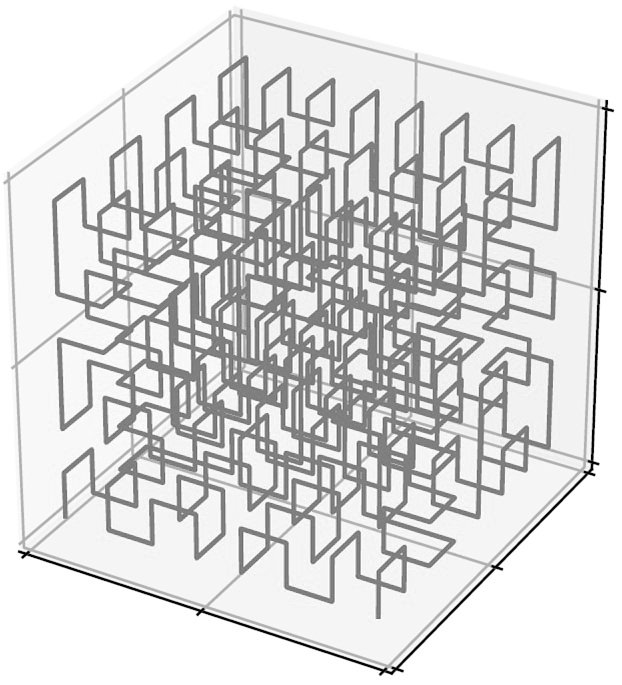
\includegraphics[width=1.0\linewidth]{fig1c.JPG} \\ (c)}
\end{minipage}
\caption{Evolvents in two dimensions with (a) $m=3$, (b) $m=4$ and (c) $m=5$}
\label{fig:0}
\end{figure}
%new text end



By using this kind of mapping it is possible to reduce the multidimensional problem~(\ref{eq:1}) to a univariate problem
\[
\varphi(y^\ast)=\varphi(y(x^\ast))=\min{\left\{\varphi(y(x)): x\in[0,1]\right\}}.
\]
An important property of such mapping is preservation of boundedness of function relative differences  (see \cite{RefStrongin2000}): if the function $\varphi(y)$ in the domain $D$ satisfies the Lipschitz condition, then the function $\varphi(y(x))$ on the interval $[0,1]$ will satisfy a uniform H{\"o}lder condition
\[
\left|\varphi(y(x_1))-\varphi(y(x_2))\right|\leq H\left|x_1-x_2\right|^{1/N},
\]
where the H{\"o}lder constant $H$ is linked to the Lipschitz constant $L$ by the relation
\[
H=4Ld\sqrt{N},\;\; d=\max{\left\{b_i-a_i:1\leq i \leq N\right\}}.
\]

Therefore, it is possible, without loss of generality, to consider minimization of univariate function
\[
f(x)=\varphi(y(x)), \;\; x\in[0,1],
\]
satisfying the H{\"o}lder condition.
%new text begin
Once again, we recall that the Peano curve $y(x)$ is defined as a limit object emerging in some sequential construction. Appropriate approximations to $y(x)$ are to be used for practical application.
%new text end

The considered algorithm for solving this problem (here, according to \cite{RefStrongin2000}) involves constructing a sequence of points $x^k$, where the values of minimized function $z^k = f(x^k)$ are calculated. Let us call the process of calculating the function value (including the construction of an image $y^k=y(x^k)$) the ``trial'', and the pair $(x^k, z^k)$, the ``trial result''. The set of pairs $\left\{(x^k, z^k)\right\}, 1\leq k\leq n,$ makes up the search data collected using the method after carrying out $n$ steps. The rules that determine the work of the global search algorithm are as follows.

At the first iteration of the method the trial is carried out at an arbitrary internal point $x^1$ of the interval $[0,1]$. The point of trial at the next iteration $(k+1)$ is determined according to the rules presented below.

Step 1. Renumber points of the set
\[
X_k=\{x^1,\dots,x^k\}\cup\left\{0\right\}\cup\left\{1\right\},
\]
which includes boundary points of the interval $[0,1]$ and the points of the previous trials, with subscripts in increasing order of coordinate values, i.e.,
\[
0=x_0<x_1<\dots <x_k<x_{k+1}=1.
\]

Step 2. Supposing that  $z_i=f(x_i), \; 1\leq i \leq k$, calculate values 
\begin{equation}\label{eq:11}
\mu = \max_{2\leq i \leq k}\frac{\left|z_i-z_{i-1}\right|}{\Delta_i},
\end{equation}
\[
M = \left\{
   \begin{array}{lr}
     r\mu, & \mu > 0,\\
     1, & \mu = 0,
   \end{array}
\right.
 \]
where $r>1$ is a preset parameter of the method, and $\Delta_i=\left(x_i-x_{i-1}\right)^{1/N}$.

Step 3. Calculate a \textit{characteristic} for every interval $(x_{i-1}, x_i), \; 1\leq i \leq k+1,$   according to the following formulae
\[
R(1)=2\Delta_1-4\frac{z_1}{M},
\]
\begin{equation}\label{eq:14}
R(i)=\Delta_i+\frac{(z_i-z_{i-1})^2}{M^2\Delta_i}-2\frac{z_i+z_{i-1}}{M},1<i<k+1,
\end{equation}
\[
R(k+1)=2\Delta_{k+1}-4\frac{z_k}{M}.
\]

Step 4. Find interval $(x_{t-1},x_t)$ with the maximum characteristic
\begin{equation}\label{eq:141}
R(t)=\max{\left\{R(i): 1 \leq i \leq k+1\right\}}.
\end{equation}

Step 5. Carry out a trial at the point $x^{k+1}\in(x_{t-1},x_t)$, calculated using the following formulae
\[
x^{k+1} = \frac{x_t+x_{t-1}}{2}, \textrm{ if } t=1 \textrm{ or } t=k+1,
\]
\begin{equation}\label{eq:142}
x^{k+1} = \frac{x_t+x_{t-1}}{2} - \mathrm{sign}(z_t-z_{t-1})\frac{1}{2r}\left[\frac{\left|z_t-z_{t-1}\right|}{\mu}\right]^N, \textrm{ if } 1<t<k+1.
\end{equation}

The algorithm terminates if the condition $\Delta_t<\epsilon$ is satisfied; here $\epsilon>0$ is the preset accuracy. For estimation of the global solution, values
\[
f_k^\ast=\min_{1\leq i \leq k}f(x^i), \ x_k^\ast=\arg \min_{1\leq i \leq k}f(x^i).
\]
are selected.

%new text begin
Remark 1. The global search algorithm was developed in the framework of a stochastic model (see \cite{RefStrongin2000}). From this point of view the normalized characteristics $R(i)$ from (\ref{eq:14}) can be considered as probabilities of locating the global minimum within the interval  $(x_{i-1},x_i), 1\leq i \leq k+1$. Thus, at each iteration a new trial point is selected inside the interval, which has the greatest probability of finding the global minimum.

Remark 2. In a different way, the global search algorithm has a geometric interpretation (see \cite{RefSergeyev2001}). Using trial points it is possible to design a support function (\textit{minorant}) for which characteristic $R(i)$ is the minimum value of the minorant in the interval $(x_{i-1},x_i), 1\leq i\leq k+1$, taken with the opposite sign. Then according to (\ref{eq:141}) new trial is carried out in the interval where the global minimizer of the current minorant is situated and the new trial point $x_{k+1}$ from (\ref{eq:142}) coincides with it.

%new text end

Remark 3. The proof of convergence of this algorithm is provided in \cite{RefStrongin2000}. The modifications taking into account existence of inequality constraints in the problem and the information about the objective function derivative are given in \cite{RefBarkalov,RefGergel1996,RefGergel1997}.

Let us illustrate the work of this \textit{global search algorithm} (GSA) using a dimension reduction for minimization of a multiextremal function of two variables 
\begin{eqnarray} \nonumber \label{eq:19}
\varphi(y)= -&\left\{\left(\sum^{7}_{i=1}\sum^{7}_{j=1}A_{ij}g_{ij}(y)+B_{ij}h_{ij}(y)\right)^2+\right. \\
&\left.\left(\sum^{7}_{i=1}\sum^{7}_{j=1}C_{ij}g_{ij}(y)+D_{ij}h_{ij}(y)\right)^2\right\}^{1/2},\\ \nonumber
\end{eqnarray}
where
\begin{eqnarray} \nonumber
& y=(y_1,y_2)\in R^2, 0 \leq y_s \leq 1, s=1,2, \\ \nonumber
& g_{ij}(y)=\sin(i\pi y_1)\sin(j\pi y_2),  \\ \nonumber
& h_{ij}(y)=\cos(i\pi y_1)\cos(j\pi y_2), \nonumber 
\end{eqnarray}
and coefficients $A_{ij}, B_{ij}, C_{ij}, D_{ij}$  are taken uniformly in the interval $[-1,1]$. The experiment used the method parameters $r=3$, $\epsilon=10^{-3}$, and the evolvent construction parameter $m=12$. Fig.~\ref{fig:1} shows the level lines of a function generated according to (\ref{eq:19}) and the points of 1103 trials carried out using the method before the required accuracy was obtained.
\begin{figure}
	\center
  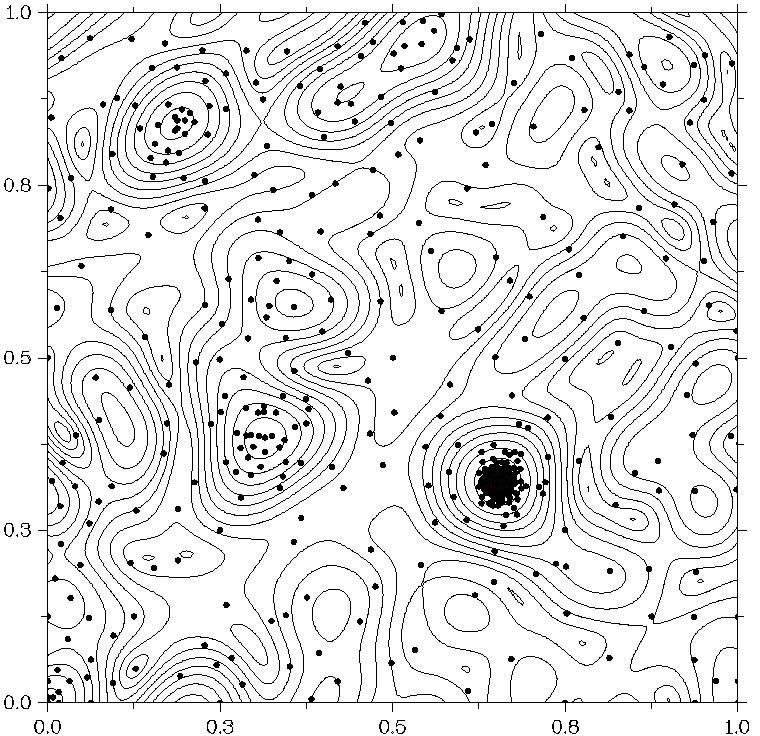
\includegraphics[width=0.75\textwidth]{fig2.jpg} 
  \caption{Minimization of a function of two variables by the sequential algorithm}
  \label{fig:1}       % Give a unique label
\end{figure}

\begin{figure}
	\center
  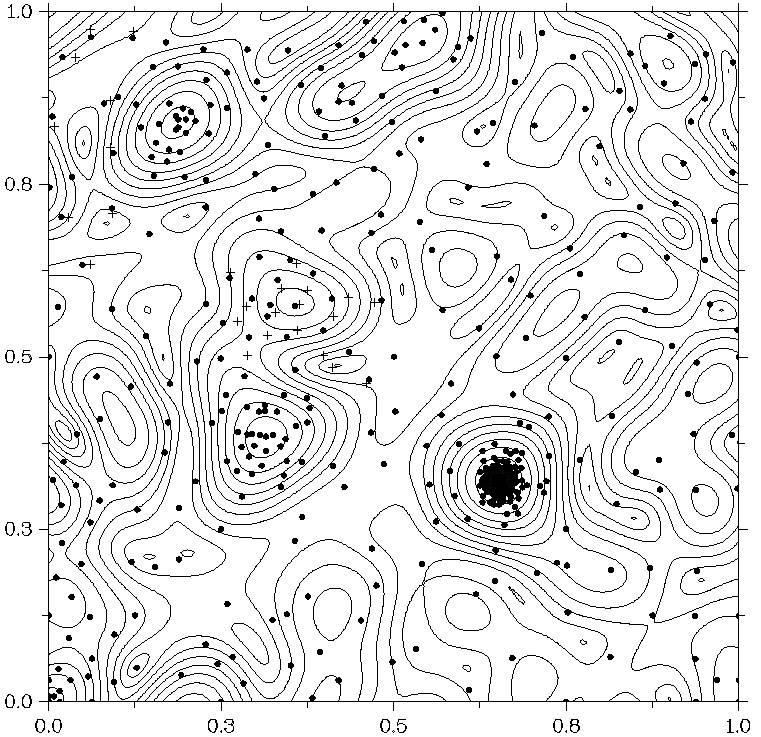
\includegraphics[width=0.75\textwidth]{fig3.jpg} 
  \caption{Minimization of a function of two variables by the parallel algorithm}
  \label{fig:2}
\end{figure}

\section{Synchronous parallel algorithm} \label{sec:3}

Let us now consider $p>1$ computing elements (cores in CPU or GPU). In this case, search process parallelization can be organized in several ways.

The first option is to parallelize calculation of the objective function describing the optimized object. This method can provide some speedup, but is specific for each problem.

The second option is to parallelize implementation of algorithm computing rules for selection of the next trial point. In this case the way of parallelization will depend on the class of algorithms. Moreover, these rules are often rather simple and it is inexpedient to parallelize them (overhead costs of the organization of parallelism will reduce possible speedup to zero).

%new text begin
The third option is to change an algorithm for the purpose of carrying out several trials in parallel. This approach is most promising since it is characterized by efficiency and generality. Firstly, the part of computing process, in which the bulk of calculations is carried out, is parallelized. Secondly, the approach is applicable for a wide class of characteristical algorithms of multiextremal optimization \cite{RefSergeyev1994,RefSergeyevGrishagin,RefGrishagin1997,RefGrishagin2001}.
%new text end

Let us describe a change of rules of global search algorithm for the case when the algorithm carries out during one iteration $p>1$ trials simultaneously (each trial on a separate processor). Let $k(n)$ be the total number of trials, carried out after $n$ parallel iterations.

Suppose $n\geq 1$  iterations of the method have been carried out, in which trials were performed at $k=k(n)$ points $x^i,1\leq i \leq k$. Then points $x^{k+1},\dots,x^{k+p}$  of search trials of the next $n+1$ iteration are determined according to the following rules.

Steps 1--3 of the parallel algorithm fully repeat steps 1--3 of the sequential global search algorithm.

Step 4. Arrange characteristics  $R(i), 1 \leq i \leq k+1$, in decreasing order 
\begin{equation}\label{eq:21}
R(t_1)\geq R(t_2)\geq \dots \geq R(t_{k}) \geq R(t_{k+1})
\end{equation}
and select $p$ maximum characteristics with interval numbers $t_j, 1\leq j \leq p$.

Step 5. Carry out new trials at points $x^{k+j}\in(x_{t_j-1},x_{t_j}), 1\leq j\leq p$, calculated using the formulae
\[
x^{k+j} = \frac{x_{t_j}+x_{t_j-1}}{2}, \textrm{ if } t_j=1 \textrm{ or } t_j=k+1,
\]
\[
x^{k+j} = \frac{x_{t_j}+x_{t_j-1}}{2} - \mathrm{sign}(z_{t_j}-z_{t_j-1})\frac{1}{2r}\left[\frac{\left|z_{t_j}-z_{t_j-1}\right|}{\mu}\right]^N, \textrm{ if } 1<t_j<k+1.
\]

The algorithm terminates if the condition $\Delta_{t_j}<\epsilon$ is satisfied at least for one number $t_j, 1 \leq j \leq p$ ; $\epsilon>0$ is the preset accuracy.  For estimation of the global solution, values
\[
f_k^\ast=\min_{1\leq i \leq k}f(x^i), \ x_k^\ast=\arg \min_{1\leq i \leq k}f(x^i).
\]
are selected.

The modifications of the parallel algorithm which takes into account the information about the minimized function derivative are given in \cite{RefGergel1999}.

This method of organizing parallel computing has the following justification \cite{RefStrongin2000,RefGrishagin1997}. The characteristics of intervals (\ref{eq:14}) used in the global search algorithm can be considered as probability measures of the global minimum point location in these intervals. Inequalities (\ref{eq:21}) arrange intervals according to their characteristics, and trials are carried out in parallel in the first $p$ intervals with the largest probabilities.

Let us use a parallel algorithm of global search for solving a problem from section \ref{sec:2} with the numbers of parallel trials $p=2$ and $p=4$. With $p=2$ the number of iterations was $569$, and the number of trials was $1138$. With $p=4$ the number of iterations was reduced to $270$, and $1080$ trials were carried out. Fig.~\ref{fig:2} shows level lines of the function with points of the trials performed by the method with $p=2$. Points of redundant trials carried out using a parallel algorithm are marked in the figure by "+". The concept of redundancy is discussed in more detail in the following section.

\section{Speedup and non-redundancy of a parallel algorithm} \label{sec:4}

Let us describe theoretical properties of a parallel algorithm, which characterize its speedup. One of the main indicators of efficiency of parallel algorithms (in any field, not only in global optimization) is a speedup in time
\[
S(p)=T(1)/T(p),
\]
where $T(1)$ is the time required to solve a problem by a sequential algorithm, and $T(p)$ is the time for solving the same problem by a parallel algorithm in a system with $p$ computing elements. The characteristic of efficiency of parallel algorithms (in relation to optimization algorithms) is also a speedup in iterations
\begin{equation}\label{eq:26}
s(p)=n(1)p/n(p),
\end{equation}
where $n(1)$ is the number of trials carried out by the sequential method, and $n(p)$ is the number of trials carried out by the parallel method with $p$ processors. This characteristic is especially important since for solving applied problems the time required to carry out a trial exceeds the time required to process its results.

It is obvious that the number of trials $n(p)$ for sequential and parallel algorithms described in sections \ref{sec:2} and \ref{sec:3} will differ. Actually, the sequential algorithm of global search when selecting point $x^{k+1}$ of the next $k+1$ trial possesses complete information received at the previous $k$ iterations. Based on the same information, the parallel algorithm of global search selects $p$ points $x^{k+j}, 1\leq j \leq p$, rather than one at iteration $k+1$. It means that selection of point $x^{k+j}$ is carried out in absence of information on the trial results at points $x^{k+i}, 1\leq i<j$. Only the first point $x^{k+1}$ will coincide with the point selected by the sequential algorithm. Other trials points generally cannot coincide with the points generated by the sequential algorithm. The efficiency owing to the use of parallel processors can be reduced when such trials are performed. Therefore, let us consider such trials as ``redundant'', and the value 
\[
\lambda(p) = \left\{
   \begin{array}{lr}
     (n(p)-n(1))/n(p), & n(p) > n(1),\\
     0, & n(p)\leq n(1),
   \end{array}
\right.
\]
will represent ``method redundancy''.

Let us set a series of trials $\left\{x^k\right\}$ and $\left\{y^m\right\}$ generated correspondingly by sequential and parallel algorithms for solving the same problem with $\epsilon = 0$ in the stopping condition. The following theorem from \cite{RefStrongin2000} determines the number of computing elements $p$, which can be involved for non-redundant parallelization.

\textbf{Theorem}. Suppose $x^\ast$ is the point of global minimum, $x'$ is the point of the local minimum of function $f(x)$, and the following conditions are fulfilled:
\begin{enumerate}
	\item
	Inequality 
	\begin{equation}\label{eq:28}
	f(x')-f(x^\ast)\leq \delta, \delta>0,
	\end{equation}
	holds.
	\item
	The initial $q(l)$ trials of the sequential and parallel methods coincide, i.e.,
	\[
	\left\{x^1,\dots,x^{q(l)}\right\}=\left\{y^1,\dots,y^{q(l)}\right\},
	\]
	where 
	\[
	\left\{x^1,\dots,x^{q(l)}\right\}\subset\left\{x^k\right\}, \ \left\{y^1,\dots,y^{q(l)}\right\}\subset\left\{y^m\right\}.
	\]
	\item
	There exists a point $y^n\in \left\{y^m\right\}, n<q(l),$ such that $x'\leq y^n \leq x^\ast$ or \mbox{$x^\ast \leq y^n \leq x'$}.
	\item
	For the value $M$ from (\ref{eq:11}) the following inequality
	\[
	M>2^{2-1/N}H
	\]
	holds, where $H$ is the H{\"o}lder constant of the minimized function.
\end{enumerate}

Then a parallel algorithm of global search using two processors will be non-redundant (i.e., $s(2)=2$, $\lambda(2)=0$) while the following condition is satisfied 
\begin{equation}\label{eq:32}
\left(x_{t_j}-x_{t_j-1}\right)^{1/N} > \frac{4\delta}{M-2^{2-1/N}H}, 1\leq j\leq p,	
\end{equation}
where $t_j$ are determined according to (\ref{eq:21}).

\textbf{Corollary}. Let the objective function $f(x)$ have $Q$ local minimum points $\left\{x'_1,\dots,x'_Q\right\}$, for which condition (\ref{eq:28}) is fulfilled, and let there exist trial points $y^{n_i}, 1\leq i \leq Q,$ such as
\[
y^{n_i}\in \left\{y^1,\dots,y^{q(l)}\right\},
\]
\[
\alpha_i \leq y^{n_i} \leq \alpha_{i+1}, \; \alpha_i, \alpha_{i+1} \in \left\{x^\ast, x'_1,\dots,x'_Q\right\}, \; 1\leq i \leq Q.
\]

Then, if the theorem conditions are satisfied, the parallel algorithm of global search with $Q+1$ processors will be non-redundant (i.e., $s(Q+1)= Q+1$, \mbox{$\lambda(Q+1)=0$}), while condition (\ref{eq:32}) is satisfied.

The theorem corollary plays a special role in solving multidimensional problems reduced to univariate problems by means of the Peano-like evolvent $y(x)$. The evolvent $y(x)$, which is an approximation to the Peano curve, has the effect of ``splitting'' of a global minimum point $y^\ast\in D$ to several preimages in the interval $[0,1]$. If function $\varphi(y)$ has the only global minimum in $D$, the ``reduced'' function $f(x)$ can have up to $2^N$ local extremum points close (by value) to a global extremum point (see \cite{RefStrongin2000}). By applying a parallel global search algorithm for minimization of a similar function it is possible to achive non-redundancy when using up to $2^N+1$ computing elements.

\begin{table}
	\caption{Results of minimization of $100$ functions of two variables}
	\label{tab:1}
	\center
	\begin{tabular}{lll}
		\hline\noalign{\smallskip}
		 $p$ & $n(p)$ & $s(p)$ \\
		\noalign{\smallskip} \hline \noalign{\smallskip}
			1 &	1575 &	\dots \\
			2 &	1596 &	1.97 \\
			3 &	1562 &	3.02 \\
			4 &	1599 &	3.94 \\
		\noalign{\smallskip}\hline
	\end{tabular}
\end{table}


The parallel algorithm of global search has demonstrated a good speedup in implementation on CPU in systems with a small number of processors. In \cite{RefGrishagin1997,RefStrongin2003} a speedup of algorithm close to linear was experimentally verified when carrying out 2-4 parallel trials. The results obtained with the parallel GSA for minimization of 100 multiextremal functions of two variables described by formula (\ref{eq:19}) are shown in table \ref{tab:1}. All experiments used method parameters $r=2.9$, and $\epsilon=10^{-3}$, and the global minimum was found with the required accuracy in all $100$ problems. The table shows the number of used processors $p$, the average number of trials $n(p)$ rounded to integers and average speedup in iterations $s(p)$ from (\ref{eq:26}). 

\section{Implementation on GPU} \label{sec:5}

What are the advantages of GPU over CPU when implementing global optimization algorithms? First, CPU has only a small (up to $16$ in the advanced models) number of cores working independently at a high clock frequency. GPU, on the contrary, works at low clock frequencies and uses hundreds of simpler computing elements. Second, a considerable part of a CPU crystal is occupied by a high-speed cache memory, while practically the whole of GPU consists of arithmetic and logic units. Therefore, GPUs are especially effective in problems, in which the number of arithmetic operations is great in comparison with memory operations.

With respect to methods of global optimization, parallel computing many values of the objective function simultaneously is an operation which can be efficiently implemented on GPU. In the function value calculation procedure implemented on GPU transfers of information from CPU to GPU will be minimal: it is necessary only to transfer the coordinates of trial points to GPU and to receive the values of the function at these points. The routines that determine the processing of trial results according to algorithm and require working with a large volume of collected search information can be efficiently implemented on CPU.

A general scheme showing the organization of calculations using GPU is given in Fig.~\ref{fig:3}. According to this scheme, steps 1 -- 4 of a parallel global search algorithm are carried out on a CPU. The coordinates of $p$ points of trials calculated at step 4 of the algorithm are collected in an intermediate buffer, and then are transferred to the graphics processing unit. Calculation of function values at these points is carried out on a GPU, and then the results of trials (again via the intermediate buffer) are transferred to the CPU.

\begin{figure}
	\center
  
\includegraphics[width=0.75\textwidth]{fig4.jpg} 
  \caption{Scheme of information exchanges in a GPU algorithm}
  \label{fig:3}
\end{figure}


The use of several hundred parallel computing elements (as in modern GPU) might not give a speedup of the search process by hundreds of times. In this case, the conditions of the theorem of non-redundant parallelization can be violated: the number of local extrema will be less than the number of computing cores. Then (according to the theorem and its corollary) a parallel GSA will generate redundant trial points. Nevertheless, despite certain redundancy, the overall operating time of a GPU algorithm will be less than the operating time of a CPU algorithm. This has been verified by computational experiments, the results of which are given in section \ref{sec:6}.

\section{Results of numerical experiments} \label{sec:6}

Computational experiments were carried out on one of the nodes of a high-performance cluster of the State University of Nizhny Novgorod. The cluster node includes 2 Intel Sandy Bridge E5-2660 2.2 GHz CPUs, 64 Gb RAM, and NVIDIA Tesla M2090 GPU. The CPU has 8 cores (i.e., 16 physical cores and 16 virtual cores in hyper-threading mode are available in the node). The graphics processing unit includes 16 multiprocessors (512 cores). For implementation of the GPU algorithm CUDA Toolkit 6.0 was used.

It should be noted that widely known test problems from the field of multidimensional global optimization are characterized by small time required to calculate the objective function value. Usually, such a calculation is nothing else than a summation of several (according to problem dimension) values of elementary functions. For example, the well known Rastrigin test function 
\begin{equation}\label{eq:33}
\varphi(y)=10N+\sum^{N}_{i=1}\left[y^2_i-10\cos(2\pi y_i)\right], \; -2.2\leq y_i \leq 1.8, \; 1\leq i \leq N,
\end{equation}
has the global minimum value $\varphi(y^\ast)=0$ at the point $y^\ast = (0,\dots,0)$.

Therefore, for the purpose of simulation of the computational complexity inherent to applied problems of optimization \cite{RefBarkalov2013}, calculation of the objective function in all performed experiments was made more complex by additional calculations without changing the type of function and arrangement of its minima (series summation from 20 thousand elements).

It is noteworthy that an important parameter for starting any GPU program (unlike a parallel program on CPU) is not only the number of threads $p$, but also the size of the \textit{thread block}. Separate threads on GPU are grouped in blocks of threads of identical size, thus each thread block is executed on a separate multiprocessor. Threads in a thread block can interact effectively using information in shared memory and synchronization. For the purpose of assessing the importance of the size of a thread block during the execution period of a GPU algorithm let us perform a preliminary series of experiments with the test function (\ref{eq:33}) with $N=5$. Let us vary the number $p$ of the used GPU threads and the size $p_b$ of a thread block. All the other parameters of the method do not change ($r=2.3$, $\epsilon = 10^{-3}$, the evolvent construction parameter $m=10$). Table \ref{tab:2} shows the GPU algorithm operating time depending on $p$ and $p_b$.
\begin{table}
	\caption{GPU algorithm operating time depending on thread block size}
	\label{tab:2}
	\center
	\begin{tabular}{llllll}
		\hline\noalign{\smallskip}
%		 $p$ & $p_b=16$ & $p_b=32$ & $p_b=64$ & $p_b=128$ & $p_b=256$  \\
		$p$ & \multicolumn{5}{l}{ \hfil $p_b$ \hfil } \\
		\noalign{\smallskip} \cline{2-6} \noalign{\smallskip}
		 & 16 & 32 & 64 & 128 & 256  \\
		\noalign{\smallskip} \hline \noalign{\smallskip}
		100 &	39.43 &	41.5 &	39.71 &	39.85 &	39.61 \\
		300 &	24.84 &	24.52 &	24.54 &	24.66 &	25.08 \\
		500 &	9.25 &	9.45 &	9.24 &	9.4 &	9.3\\
		700 &	11.8 &	13.43 &	11.78 &	11.91 &	12.03\\
		900 &	10.9 &	10.91 &	10.85 &	10.86 &	10.96\\
		1000 &	10.92 &	10.8 &	10.76 &	10.9 &	10.74\\
		\noalign{\smallskip}\hline
	\end{tabular}
\end{table}

As it seen from this table, there is a speedup of the algorithm in the case of an increase in the number of trials at one iteration up to the number of cores on GPU, with subsequent saturation. Owing to a weak information dependence the size of the thread block $p_b$ does not have decisive effect, therefore let us use $p_b=64$ in all subsequent experiments. When carrying out this set of experiments the load on GPU was 15 -- 85 \% (depending on the number of threads); the load was measured by GPUZ program.

After the parameters of the GPU algorithm have been determined let us make the main computational experiments on a series of multidimensional multiextremal problems. In work \cite{RefGaviano} a GKLS generator allowing generation of multiextremal optimization problems with known properties (number of local minima, size of their domains of attraction, global minimum point, etc.) is described.  

The results of numerical comparison of three sequential algorithms -- DIRECT \cite{RefJones}, DIRECT\textit{l} \cite{RefGablonsky} and global search algorithm (GSA) from section \ref{sec:2} -- are provided below (results of the work of the first two algorithms are given in paper \cite{RefGaviano}). Numerical comparison was carried out on function classes \textit{Simple} and \textit{Hard} of dimension 4 and 5 from \cite{RefGaviano} since solving a problems of dimension 2 and 3 demands a small number of iterations and it is impractical to use GPU for solving these problems. Global minimum $y^\ast$ was considered to be found, if the algorithm generated trial point $y^k$ in $\delta$-vicinity of the global minimum, i.e., $\left\|y^k-y^\ast\right\|\leq\delta$. The size of the vicinity was selected (according to \cite{RefGaviano}) as $\delta = \left\|b-a\right\|\sqrt[N]{\Delta}$, $N$ -- problem dimension, $a$ and $b$ -- borders of search domain $D$, parameter $\Delta=10^{-6}$ at $N=4$ and $\Delta=10^{-7}$ at $N=5$. When using the GSA for the class \textit{Simple} parameter $r=4.5$ was selected, for the class \textit{Hard} $r=5.6$ was selected; evolvent construction parameter was fixed as $m=10$. The maximum allowable number of iterations was $K_{max} = 10^6$.

The average number of iterations $k_{av}$ performed by the method for solving a series of problems from these classes is shown in table \ref{tab:3}. Symbol ''$>$''  reflects a situation in which not all problems of the class were solved by the method. This means that the algorithm was stopped as the maximum allowable number of iterations $K_{max}$ was achieved. In this case, value $K_{max}=10^6$ was used for calculating the average value of the number of iterations $k_{av}$ that corresponds to the lower estimate of this average value. The number of unsolved problems is specified in brackets.

\begin{table}
	\caption{Average number of iterations $k_{av}$}
	\label{tab:3}
	\center
	\begin{tabular}{lllll}
		\hline\noalign{\smallskip}
  	 $N$ & Problem class & DIRECT & DIRECT\textit{l} & GSA \\
		\noalign{\smallskip} \hline \noalign{\smallskip}
			4 &	\textit{Simple}	& $>$47282(4) &	18983 &	11953 \\
	      & \textit{Hard} &	$>$95708(7) &	68754 &	25263 \\
			5	& \textit{Simple} &	$>$16057(1) &	16758 &	15920 \\
				& \textit{Hard} &	$>$217215(16) &	$>$269064(4) & $>$148342(4) \\
		\noalign{\smallskip}\hline
	\end{tabular}
\end{table}

Table \ref{tab:3} shows that GSA outperforms DIRECT and DIRECT\textit{l} methods on all classes of problems in terms of average number of iterations. In class 5-\textit{Hard} all three methods failed to solve all problems: DIRECT did not solve 16 problems, DIRECT\textit{l} and GSA, 4 problems.

Let us estimate now the speedup when using the parallel global search algorithm implemented on CPU depending on the number $p$ of the used cores. Table \ref{tab:4} shows the average number of iterations performed by the method when solving a series of problems, and table \ref{tab:5} shows the average time required to solve one problem. Tables \ref{tab:6} and \ref{tab:7} show speedup in time $S(p)$ and iterations $s(p)$, respectively; speedup of the parallel algorithm was measured in relation to the sequential one ($p=1$).

\begin{table}
	\caption{Average number of iterations on CPU}
	\label{tab:4}
	\center
	\begin{tabular}{llllll}
		\hline\noalign{\smallskip}
		$p$ & \multicolumn{2}{l}{ $N=4$ } & & \multicolumn{2}{l}{$N=5$} \\
		\noalign{\smallskip} \cline{2-3} \cline{5-6} \noalign{\smallskip}
		 & \textit{Simple} & \textit{Hard} & & \textit{Simple} & \textit{Hard}  \\
		\noalign{\smallskip} \hline \noalign{\smallskip}
		1 &	11953 &	25263 & &	15920 &	$>$148342(4) \\
		2 &	6014 &	16509 & & 17797 &	98667 \\
		4 &	2547 &	8970 & &	8246 &	45410 \\
		8 &	1413 &	4666 & &	3773 &	26732 \\
		16 &	756 &	1910 & &	1713 &	11322 \\
		32 &	323 &	1252 & &	781 &	11745 \\
		\noalign{\smallskip}\hline
	\end{tabular}
\end{table}

\begin{table}
	\caption{Average problem solution time on CPU}
	\label{tab:5}
	\center
	\begin{tabular}{llllll}
		\hline\noalign{\smallskip}
		$p$ & \multicolumn{2}{l}{ $N=4$ } & & \multicolumn{2}{l}{$N=5$} \\
		\noalign{\smallskip} \cline{2-3} \cline{5-6} \noalign{\smallskip}
		 & \textit{Simple} & \textit{Hard} & & \textit{Simple} & \textit{Hard}  \\
		\noalign{\smallskip} \hline \noalign{\smallskip}
		1 &	3.02 &	6.05 & &	4.84 &	$>$42.5 \\
		2 &	1.8 &	4.48 & &	5.84 &	33.77 \\
		4 &	1.0 &	2.94 & &	3.18 &	15.62 \\
		8 &	0.71 &	1.88 & &	1.82 &	14.16 \\
		16 &	0.57 &	1.36 & &	1.44 &	8.37 \\
		32 &	0.38 &	1.25 & &	0.95 &	11.67 \\
		\noalign{\smallskip}\hline
	\end{tabular}
\end{table}

\begin{table}
	\caption{Time speedup $S(p)$ on CPU}
	\label{tab:6}
	\center
	\begin{tabular}{llllll}
		\hline\noalign{\smallskip}
		$p$ & \multicolumn{2}{l}{ $N=4$ } & & \multicolumn{2}{l}{$N=5$} \\
		\noalign{\smallskip} \cline{2-3} \cline{5-6} \noalign{\smallskip}
		 & \textit{Simple} & \textit{Hard} & & \textit{Simple} & \textit{Hard}  \\
		\noalign{\smallskip} \hline \noalign{\smallskip}
		2 &	1.68 &	1.35 & &	0.83 &	$>$1.26 \\
		4 &	3.04 &	2.06 & &	1.52 &	2.72 \\
		8 &	4.27 &	3.22 & &	2.66 &	3.64 \\
		16 &	5.29 &	4.46 & &	3.36 &	5.08 \\
		32 &	8.04 &	4.85 & &	5.11 &	3.0 \\
		\noalign{\smallskip}\hline
	\end{tabular}
\end{table}


\begin{table}
	\caption{Iteration speedup $s(p)$ on CPU}
	\label{tab:7}
	\center
	\begin{tabular}{llllll}
		\hline\noalign{\smallskip}
		$p$ & \multicolumn{2}{l}{ $N=4$ } & & \multicolumn{2}{l}{$N=5$} \\
		\noalign{\smallskip} \cline{2-3} \cline{5-6} \noalign{\smallskip}
		 & \textit{Simple} & \textit{Hard} & & \textit{Simple} & \textit{Hard}  \\
		\noalign{\smallskip} \hline \noalign{\smallskip}
		2 &	1.99 & 1.53 & &	0.89 &	$>$1.50 \\
		4 &	4.69 &	2.82 & &	1.93 &	3.27 \\
		8 &	8.46 &	5.41 & &	4.22 &	5.55 \\
		16 &	15.82 &	13.23 & &	9.29 &	13.1 \\
		32 &	37.04 &	20.18 & &	20.39 &	12.63 \\
		\noalign{\smallskip}\hline
	\end{tabular}
\end{table}

\begin{table}
	\caption{Redundancy $\lambda(p)$ on CPU}
	\label{tab:8}
	\center
	\begin{tabular}{llllll}
		\hline\noalign{\smallskip}
		$p$ & \multicolumn{2}{l}{ $N=4$ } & & \multicolumn{2}{l}{$N=5$} \\
		\noalign{\smallskip} \cline{2-3} \cline{5-6} \noalign{\smallskip}
		 & \textit{Simple} & \textit{Hard} & & \textit{Simple} & \textit{Hard}  \\
		\noalign{\smallskip} \hline \noalign{\smallskip}
2 &	0.01 & 0.23 & &	0.55 &	$>$0.25 \\
4 &	0 &	0.3 & &	0.52	& 0.18 \\
8 &	0 &	0.32 & &	0.47  &	0.31 \\
16 &	0.01 &	0.17& &	0.42  &	0.18 \\
32 &	0 &	0.37 & &	0.36  &	0.61 \\
		\noalign{\smallskip}\hline
	\end{tabular}
\end{table}

The data show fivefold time speedup, when using 32 cores for all classes (except 5-\textit{Hard}). The lack of expected speedup in class 5-\textit{Hard} in transition from 16 to 32 cores is explained by an increase in the average number of iterations and by the fact that of 32 cores 16 are physical, and other 16 are virtual in hyper-threading mode, i.e., a real gain in performance in transition from 16 to 32 cores is less than twofold.

Let us make a similar experiment using a GPU version of the algorithm. Also let us fix the average number of iterations and average time required to solve one problem (see tables \ref{tab:last4} -- \ref{tab:last}). Let us measure the speedup and redundancy of GPU algorithm in relation to the CPU algorithm started with 32 cores (see column $p=32$ in tables \ref{tab:4} and \ref{tab:5}). The number of the used threads $p$ on GPU varied, all other parameters of the method did not change. The number of threads, which is greater than the number of cores, was chosen to show the following effect: the number of iterations executed by the algorithm will be reduced in case of an increase of the threads number, while the algorithm operation time will not be reduced. The minimum time of operation is reached, if the number of used threads does not surpass the number of GPU cores.


\begin{table}
	\caption{Average number of iterations on GPU}
	\label{tab:last4}
	\center
	\begin{tabular}{llllll}
		\hline\noalign{\smallskip}
		$p$ & \multicolumn{2}{l}{ $N=4$ } & & \multicolumn{2}{l}{$N=5$} \\
		\noalign{\smallskip} \cline{2-3} \cline{5-6} \noalign{\smallskip}
		 & Simple & Hard & & Simple & Hard  \\
		\noalign{\smallskip} \hline \noalign{\smallskip}		
100 &	105 &	352 & &	193  &	2452 \\
200 &	56 &	181 & &	105  &	809 \\
300 &	53 &	107 & & 62  &	508 \\
400 &	28 &	87 & &	44  &	376 \\
500 &	24 &	84 & &	41  &	353 \\
800 &	18 &	37 & &	55 &	246 \\
1000 &	12 &	33 & &	36 &	172 \\
		\noalign{\smallskip}\hline
	\end{tabular}
\end{table}


\begin{table}
	\caption{Average problem solution time on GPU}
	\label{tab:last3}
	\center
	\begin{tabular}{llllll}
		\hline\noalign{\smallskip}
		$p$ & \multicolumn{2}{l}{ $N=4$ } & & \multicolumn{2}{l}{$N=5$} \\
		\noalign{\smallskip} \cline{2-3} \cline{5-6} \noalign{\smallskip}
		 & Simple & Hard & & Simple & Hard  \\
		\noalign{\smallskip} \hline \noalign{\smallskip}		
		100  & 0.16 &	0.5 & &	0.33 & 3.46 \\
		200 &	0.16 &	0.47 & &	0.32  &	2.11 \\
		300 &	0.22 &	0.43 & &	0.29  &	1.98 \\
		400 &	0.16 &	0.44 & &	0.27  &	1.97 \\
		500 &	0.16 &	0.52 & &	0.31 &	2.25 \\
		800 &	0.19 &	0.37 & &	0.6 &	2.54 \\
		1000 &	0.15 &	0.41 & &	0.48  &	2.15 \\
		\noalign{\smallskip}\hline
	\end{tabular}
\end{table}


\begin{table}
	\caption{Time speedup $S(p)$ on GPU}
	\label{tab:last2}
	\center
	\begin{tabular}{llllll}
		\hline\noalign{\smallskip}
		$p$ & \multicolumn{2}{l}{ $N=4$ } & & \multicolumn{2}{l}{$N=5$} \\
		\noalign{\smallskip} \cline{2-3} \cline{5-6} \noalign{\smallskip}
		 & Simple & Hard & & Simple & Hard  \\
		\noalign{\smallskip} \hline \noalign{\smallskip}		
		100 &	2.3  &	2.49 & &	2.9  &	4.09 \\
		200 &	2.35 &	2.68 & &	2.99 &	6.72 \\
		300 &	1.75 &	2.93 & &	3.32 &	7.17 \\
		400 &	2.37 &	2.85 & &	3.58 &	7.19 \\
		500 &	2.38 &	2.41 & &	3.05 &	6.3 \\
		800 &	1.94 &	3.38 & &	1.59 &	5.56 \\
		1000 & 2.45 &	3.07 & &	1.98 &	6.59 \\				
		\noalign{\smallskip}\hline
	\end{tabular}
\end{table}



\begin{table}
	\caption{Iteration speedup $s(p)$ on GPU}
	\label{tab:last1}
	\center
	\begin{tabular}{llllll}
		\hline\noalign{\smallskip}
		$p$ & \multicolumn{2}{l}{ $N=4$ } & & \multicolumn{2}{l}{$N=5$} \\
		\noalign{\smallskip} \cline{2-3} \cline{5-6} \noalign{\smallskip}
		 & Simple & Hard & & Simple & Hard  \\
		\noalign{\smallskip} \hline \noalign{\smallskip}
		100	&	3.07	&	3.55	& &	4.05	&	4.79	\\
		200	&	5.78	&	6.90	& &	7.45	&	14.51	\\
		300	&	6.11	&	11.70	& &	12.57	&	23.12	\\
		400	&	11.43	&	14.38	& &	17.80	&	31.21	\\
		500	&	13.54	&	14.98	& &	18.83	&	33.26	\\
		800	&	17.96	&	33.46	& &	14.19	&	47.68	\\
		1000	&	27.42	&	37.40	& &	21.91	&	68.21	\\
		\noalign{\smallskip}\hline
	\end{tabular}
\end{table}


\begin{table}
	\caption{Redundancy $\lambda(p)$ on GPU}
	\label{tab:last}
	\center
	\begin{tabular}{llllll}
		\hline\noalign{\smallskip}
		$p$ & \multicolumn{2}{l}{ $N=4$ } & & \multicolumn{2}{l}{$N=5$} \\
		\noalign{\smallskip} \cline{2-3} \cline{5-6} \noalign{\smallskip}
		 & Simple & Hard & & Simple & Hard  \\
		\noalign{\smallskip} \hline \noalign{\smallskip}
		100 & 0.02 & 0.0 & & 0.0 & 0.0  \\
		200 & 0.08 & 0.0 & & 0.0 & 0.0  \\
		300 & 0.35 & 0.0 & & 0.0 & 0.0  \\
		400 & 0.09 & 0.0 & & 0.0 & 0.0  \\
		500 & 0.13 & 0.04 & & 0.0 & 0.0  \\
		800 & 0.28 & 0.0 & & 0.43 & 0.0  \\
		1000 & 0.12 & 0.0 & & 0.3 & 0.0  \\
		\noalign{\smallskip}\hline
	\end{tabular}
\end{table}

The results of our experiments show some obvious advantages of the GPU algorithm in comparison with the CPU algorithm. The algorithm, which uses the maximal number of cores of CPU, works slower than any of the given GPU implementations. In addition, the results show a considerable decrease of the number of iterations. For example, on average only 353 parallel iterations on GPU were sufficient to solve problems of the most difficult class considered -- 5-\textit{Hard}, whereas even with the use of all computing CPU cores over eleven thousand iterations were required. Finally, the GPU algorithm is almost non-redundant in relation to the CPU algorithm.

\section{Conclusions} \label{sec:7}

Summing up the results, let us note that use of graphics processing units for solving global optimization problems is a new, promising line of research as high efficiency of modern supercomputers is reached (generally) due to the use of graphics accelerators. 

This paper considers a parallel algorithm for solving multidimensional multiextremal optimization problems and its implementation on GPU. This algorithm was developed within the framework of information-statistical approach. Theoretical information on the properties of the parallel algorithm characterizing the conditions of non-redundant parallelization are provided.

For the purpose of experimental demonstration of theoretical properties of the considered parallel algorithms, computational experiments on a series of several hundred test problems of different dimensions were performed. The results obtained with the sequential global search algorithm show its superiority over several known methods of global optimization. At the same time the parallel algorithm shows a good speedup and low redundancy (both GPU and CPU version), and the GPU version of the parallel algorithm shows a speedup of 2 to 6 times in comparison with the fastest parallel CPU version.

\begin{acknowledgements}

The authors of the paper express their gratitude to Ilya Lebedev for assistance in carrying out the computational experiments.

\end{acknowledgements}

% BibTeX users please use one of
%\bibliographystyle{spbasic}      % basic style, author-year citations
%\bibliographystyle{spmpsci}      % mathematics and physical sciences
%\bibliographystyle{spphys}       % APS-like style for physics
%\bibliography{}   % name your BibTeX data base

% Non-BibTeX users please use
\begin{thebibliography}{}

\bibitem{RefPinter}
Pinter, J.D. (ed.): Global Optimization: Scientific and Engineering Case Studies. Springer (2006).

\bibitem{RefHwu}
Hwu, W.: GPU Computing Gems Emerald Edition (Applications of GPU Computing Series). Morgan Kaufmann (2011).

\bibitem{RefApuzzo}
D'Apuzzo, M.,  Marino, M., Migdalas, A., Pardalos, P.M., Toraldo, G.: Parallel computing in global optimization. In Handbook of Parallel Computing and Statistics, Chapman \& Hall, London, 225--258 (2006)

\bibitem{RefFerreiro}
Ferreiro, A.M., Garcia, J.A., Lopez-Salas, J.G., Vazquez, C.: An efficient implementation of parallel simulated annealing algorithm in GPUs. J. Glob. Optim. 57(3), 863--890 (2013)

\bibitem{RefZhu}
Zhu, W.: Massively parallel differential evolution--pattern search optimization with graphics hardware acceleration: an investigation on bound constrained optimization problems. J. Glob. Optim. 50(3), 417--437 (2011).

\bibitem{RefGarcia}
Garcia-Martinez, J.M., Garzon, E.M., Ortigosa, P.M.: A GPU implementation of a hybrid evolutionary algorithm: GPuEGO. J. Supercomput. (2014) doi:10.1007/s11227-014-1136-7 

\bibitem{RefMussi}
Mussi, L., et al.: GPU implementation of a road sign detector based on particle swarm optimization. Evol. Intel. 3 (3), 155--169 (2010)

\bibitem{RefLangdon}
Langdon, W.B.: Graphics processing units and genetic programming: an overview. Soft. Comput. 15(8), 1657--1669 (2011)

\bibitem{RefGergel2005}
Gergel, V.P., Strongin, R.G.: Parallel computing for globally optimal decision making on cluster systems. Future Generation Computer Systems, 21(5), 673--678 (2005)

\bibitem{RefEvtushenko}
Evtushenko, Yu.G., Malkova, V.U., Stanevichyus, A.A.: Parallel global optimization of functions of several variables. Computational Mathematics and Mathematical Physics, 49(2), 246--260 (2009)

\bibitem{RefHe}
He, J., Verstak, A., Watson, L.T., Sosonkina, M.: Design and implementation of a massively parallel version of DIRECT. Comput. Optim. Appl. 40(2), 217--245 (2008)

\bibitem{RefPaulavicius}
Paulavicius, R., Zilinskas, J., Grothey, A.: Parallel branch and bound for global optimization with combination of Lipschitz bounds. Optimization Methods \& Software 26(3), 487--498, (2011)

\bibitem{RefBoukedjar}
Boukedjar A., Lalami M. E., El Baz D.: Parallel Branch and Bound on a CPU-GPU System. In 20th Int. Conf. on Parallel,  Distributed and Network-Based Processing, 392--398 (2012)

\bibitem{RefCarneiro}
Carneiro, T. et al.: A new parallel schema for branch-and-bound algorithms using GPGPU. In 23rd Int. Symposium on Computer Architecture and High Performance Computing, 41--47 (2011)

\bibitem{RefKindratenko}
Kindratenko, V. (ed.): Numerical Computations with GPUs. Springer (2014).

\bibitem{RefStrongin2000}
Strongin, R.G., Sergeyev, Ya.D.: Global optimization with non-convex constraints. Sequential and parallel algorithms. Kluwer Academic Publishers, Dordrecht (2000)

\bibitem{RefLebedevBarkalov}
Lebedev, I.G., Barkalov, K.A.: A GPU implementation of a parallel global search algorithm. PNRPU Aerospace Engineering Bulletin 36, 64--82 (2014) (in Russian)

\bibitem{RefSergeyev2006}
Sergeyev Ya.D., Kvasov D.E.: Global search based on efficient diagonal partitions and a set of Lipschitz constants. SIAM J. Optim. 16(3), 910--937 (2006)

\bibitem{RefZilinskas}
Zilinskas, J.: Branch and bound with simplicial partitions for global optimization. Mathematical Modelling and Analysis 13(1), 145--159 (2008)

\bibitem{RefSergeyev2013}
Sergeyev, Ya.D., Strongin, R.G., Lera, D.: Introduction to global optimization exploiting space-filling curves. Springer (2013)

\bibitem{RefSergeyev2001}
Molinaro, A., Pizzuti, C., and Sergeyev, Ya.D.: Acceleration tools for diagonal information global optimization algorithms. Computational Optimization and Applications 18, 5--26 (2001)

\bibitem{RefBarkalov}
Barkalov, K.A., Strongin, R.G.: A global optimization technique with an adaptive order of checking for constraints. Computational Mathematics and Mathematical Physics 42(9), 1289--1300 (2002)

\bibitem{RefGergel1996}
Gergel, V.P.: A method of using derivatives in the minimization of multiextremum functions. Computational Mathematics and Mathematical Physics 36(6), 729--742 (1996)

\bibitem{RefGergel1997}
Gergel, V.P.: A global optimization algorithm for multivariate functions with lipschitzian first derivatives. J. Glob. Optim.10(3), 257--281 (1997)

\bibitem{RefSergeyev1994}
Sergeyev, Ya.D., Grishagin, V.A.: A parallel method for finding the global minimum of univariate functions. J. Optim. Theory Appl. 80(3), 513--536 (1994)

\bibitem{RefSergeyevGrishagin}
Sergeyev, Ya.D., Grishagin, V.A.:  Sequential and parallel global optimization algorithms. Optimization Methods and Software. 3, 111--124 (1994)

\bibitem{RefGrishagin1997}
Grishagin, V.A., Sergeyev, Ya.D., Strongin, R.G.: Parallel characteristical algorithms for solving problems of global optimization. J. Glob. Optim. 10(2), 185--206 (1997)

\bibitem{RefGrishagin2001}
Sergeyev Ya.D, Grishagin V.A.: Parallel asynchronous global search and the nested optimization scheme. Journal of Computational Analysis and Applications. 3(2), 123--145 (2001)

\bibitem{RefGergel1999}
Gergel, V.P., Sergeyev, Ya.D.: Sequential and parallel algorithms for global minimizing functions with Lipschitzian derivatives. Computers and Mathematics with Applications, 37(4-5), 163--179 (1999)

\bibitem{RefStrongin2003}
Strongin, R.G., Sergeyev, Ya.D.: Global optimization: fractal approach and non-redundant parallelism. J. Glob. Optim. 27(1), 25--50 (2003)

\bibitem{RefBarkalov2013}
Barkalov, K., Polovinkin, A., Meyerov, I., Sidorov, S., Zolotykh, N.: SVM regression parameters optimization using parallel global search algorithm // Lecture Notes in Computer Science. 7979, 154--166 (2013)

\bibitem{RefGaviano}
Gaviano, M., Lera, D., Kvasov, D.E., Sergeyev, Ya.D.: Software for generation of classes of test functions with known local and global minima for global optimization. ACM Trans. Math. Software 29, 469--480 (2003)

\bibitem{RefJones}
Jones, D.R., Perttunen, C.D., Stuckman, B.E.: Lipschitzian optimization without the lipschitz constant. J. Optim. Theory Appl. 79(1), 157--181 (1993)

\bibitem{RefGablonsky}
Gablonsky, J.M., Kelley, C.T.: A locally-biased form of the DIRECT algorithm. J. Glob. Optim., 21(1), 27--37 (2001)

%10.	V. Gergel, V. Grishagin, R. Israfilov, Local Tuning in Nested Scheme of Global Optimization, Procedia Computer Science 51, pp. 865–874, 2015.

\end{thebibliography}

\end{document}
